% !TEX root = ../thesis.tex

The state of the art in image processing has changed when graphics processing units (GPU) were used to train neural networks. GPUs contain many cores, they have very large data bandwidth and they are optimized for efficient matrix operations. In 2012, \cite{krizhevsky2012imagenet} used two GPUs to train an 8 layer convolutional neural network (CNN). With this model, they won the ImageNet Large Scale Visual Recognition Competition (ILSVRC) classification task (\cite{deng2012image}). Their model has improved the previous (top-5) classification accuracy record from $\sim 74\%$ to $\sim 84\%$. This caused a big trend shift in computer vision. 

As the years passed, GPUs got more and more powerful. In 2012, \cite{krizhevsky2012imagenet} used GPUs that had 3 GB memory each. Today there are GPUs with up to 16 GB memory. The number of floating point operations per second (FLOPs) has also increased from $2.5$ tera FLOPs (TFLOPs) to $12$ TFLOPs. This gradual but steep change has allowed the use of more layers and more parameters. For example, \cite{Simonyan:2014aa} introduced a model called VGGNet. Their model used up to 19 layers and showed that deeper models achieve better accuracy. \cite{He:2015aa} introduced a new method called residual connections, that allowed the use of up to 200 layers. Building up on such models, in 2016 ILSVRC winning (top-5) classification accuracy has increased to $\sim 97\%$. 

In contrast, \cite{Szegedy:2014aa} have shown that incorporating layers to compose blocks (i.e. inception blocks) works better than stacking layers. Their proposal has also been supported by \cite{Canziani:2016aa}. \cite{Canziani:2016aa} has shown the relationship between the number of parameters and the top-1 classification accuracy of state of the art models trained on ILSVRC dataset. They compare Inception-v3 (\cite{Szegedy_2016_CVPR}) and ResNet-152 (\cite{He:2015aa}) in terms of accuracy and number of parameters, and show that Inception-v3, while having fewer layers, fewer parameters and requiring a smaller number of floating point operations, performs better than ResNet-152. Their results reveal that, providing more layers and parameters does not necessarily yield better results.

ILSVRC is one of the most famous competitions in image processing. Every year, the winners of this competition are driving the research in the field. However, this competition is not considering the computational cost of solutions. The computational cost is an important factor to express the cost of real life applications of a model. For example, the 2016 winner of ILSVRC, used an ensemble of large models\footnote{\url{http://image-net.org/challenges/LSVRC/2016/results\#team}}. Such an ensemble is very expensive to use in real life because of its high computational cost. But because the cost is hidden, these results are creating an unreal expectation in public. It looks like these methods are applicable without a cost. In this thesis, we try to come up with some methods that can be used to create state of the art solutions that could easily be applicable in real life. % To define \textit{applicable in real life}, we benchmark our solution on mobile devices. These devices are affordable and they have great availability, we believe that it is a proper platform for bridging the gap between expectations of the public and reality. In this thesis, we will answer,

\begin{quote}
How can we reduce the computational cost of inference in convolutional neural networks without compromising on accuracy?
\end{quote}

First, we will briefly describe neural networks and some underlying concepts. We will mention the computational cost of necessary operations. In chapter two we will explain some methods to reduce the computational cost and run experiments on these methods. We also design and train some convolutional neural networks designed to have less computational cost. In chapter three, we will present the results of our experiments. In chapter four, we will retrospect to our decisions, experiment design, results. In chapter five, we will conclude our research and answer the research question.


\section{Notations}
We will be dealing with tensors of various shapes. Therefore we will be defining a notation that will help us through the process. We will define ordered sets to group semantically similar elements and to represent the $k$th element of such a set we will use superscript variables, such as $\wk{k}$. Since these sets represent a semantic group of variables that may have different properties, such as shape, dimensions or type, it would be misleading to represent them using a global tensor. We will not be separating scalars, vectors, matrices or tensors using capitals or bolds. However, we will be reminding the definition of these variables whenever we find necessary. We will use the $\wk{k} \inreal{5 \times 5}$ notation to state that $\wk{k}$ is a $5 \times 5$ matrix with real numbers as values. To describe the coordinates of a variable, we will use subscript variables. We use $\wki{k}{i,j}$ to represent the $i$th column and $j$th row of the matrix $\wk{k}$. We use commas or parentheses to group these variables or dimensions semantically. 
\section{Neural Networks}
In this section, we will describe neural networks briefly, provide some terminology and give some examples. 

Neural networks are \textit{weighted graphs}. They consist of an ordered set of \textit{layers}, where every layer is a set of \textit{nodes}. The first layer of the neural network is called the \textit{input layer}, and the last one is called the \textit{output layer}. The layers in between are called \textit{hidden layers}. Layers are a semantic group of nodes. Nodes belonging to one layer are connected to the nodes in the following and/or the previous layers. These connections are weighted edges, and they are referred to as \textit{weights}. 

Given an input, neural network nodes have \textit{outputs}, which are real numbers. The output of a node is calculated by applying a function ($\lf$) to the outputs of the nodes belonging to previous layers. Preceding that, the output of the input layer ($\ok{0}$) is equal to the input (see Eq. \ref{eq:output_of_layers}).  By calculating the layer outputs consecutively we calculate the output of the output layer. This process is called \textit{inference}. We use the following notations to denote the concepts that we just explained.
\begin{equation*}
\begin{split}
\num\layer & \text{: the number of layers in a neural network}\\
\lk{k} & \text{: layer $k$}\\
\mk{k} & \text{: the number of nodes in $\lk{k}$}\\
\lki{k}{i}  & \text{: node $i$ in $\lk{k}$}\\
\ok{k}  & \text{: the output vector representing the outputs of nodes in $\lk{k}$}\\
\oki{k}{i}  & \text{: the output of $\lki{k}{i}$}\\
\wk{k}  & \text{: weight matrix connecting nodes in $\lk{k-1}$ to nodes in $\lk{k}$} \\
\wki{k}{i,j}  & \text{: the weight connecting nodes $\lki{k-1}{i}$ and $\lki{k}{j}$} \\
\bk{k}  & \text{: the bias vector for $\lk{k}$} \\
\lfk{k} & \text{: function to determine $\ok{k}$ given $\ok{k-1}$}\\
\act & \text{: activation function} \\
\all\x & \text{: all inputs of the dataset as}\\
\all\y & \text{: all provided outputs of the dataset} \\
\all\yh & \text{: approximations of all outputs given all inputs}  \\
\xn{n} & \text{: $n$th input data} \\
\yn{n} & \text{: $n$th output data} \\
\yhn{n} & \text{: approximation of $\yn{n}$ given $\xn{n}$}
\end{split}
\end{equation*}

Therefore, the structure of a neural network is determined by the number of layers and the functions that determine the outputs of layers.
\begin{equation}
\label{eq:output_of_layers}
    \ok{k} = 
\begin{cases}
    \lfk{k}(\ok{k-1}), &\text{if } k\geq 1\\
    \xn{n},& k = 0\\
\end{cases}
\end{equation}


\subsection{Fully Connected Layers}
As the name suggests, for two consecutive layers to be \textit{fully connected}, all nodes in the previous layer must be connected to all nodes in the following layer. 

Let us assume two consecutive layers, $\lk{k-1} \inreal{\mk{k-1} \times 1}$ and $\lk{k} \inreal{\mk{k} \times 1}$. For these layers to be fully connected, the weight matrix connecting them would be defined as $\wk{k} \inreal{\mk{k-1} \times \mk{k}}$. This structure is represented in Figure~\ref{fig:fully_connected}.

Most fully connected layers also include a bias term ($\bk{k} \in  \real{\mk{k}}$) to account for the constants in the system. Using the weight and the bias, the output of a fully connected layer, $\ok{k}$, would simply be calculated using layer function $\FC$ as
$$ \ok{k} = \FCk{k}(\ok{k-1}) = (\ok{k-1})^T \wk{k} + \bk{k}$$
The computational complexity of $\FCk{k}$ is
$$\bigo{\FCk{k}} = \bigo{\mk{k-1}\mk{k}}$$

\begin{figure}[!h]
  \begin{centering}
    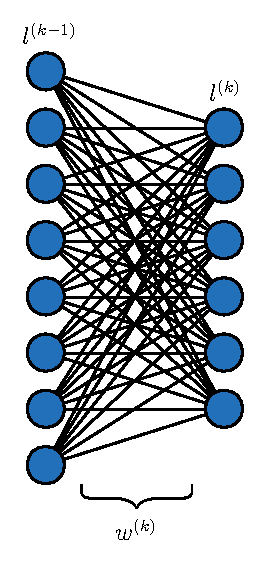
\includegraphics[width=.3\textwidth]{images/fully_connected.pdf}
    \caption{Graph representation of two fully connected layers, $\lk{k-1}$ and $\lk{k}$, connected by the weight matrix $\wk{k}$.}
    \label{fig:fully_connected}
  \end{centering}
\end{figure}

\subsection{Activation Function and Nonlinearity}
By stacking fully connected layers, we can increase the depth of a neural network. By doing so we may be able to increase approximation quality of the neural network. However, the $\FC$ we have defined is a linear function. Therefore, no matter how many linear fully connected layers we stack, we would end up with a linear model.

To achieve non-linearity, we apply \textit{activation functions} to the results of $\lf$. There are many activation functions (such as $tanh$ or $sigmoid$) but one very commonly used activation function is $\RELU$ \cite{nair2010rectified}. As shown in Figure~\ref{fig:relu}, $\RELU$ is defined as
\begin{equation}
\label{eq:relu_definition}
    \RELU(x) = 
\begin{cases}
    x, & \text{if }x \geq 0\\
    0 &  \text{otherwise }\\
\end{cases}
\end{equation}
\begin{figure}[!h]
  \begin{centering}
    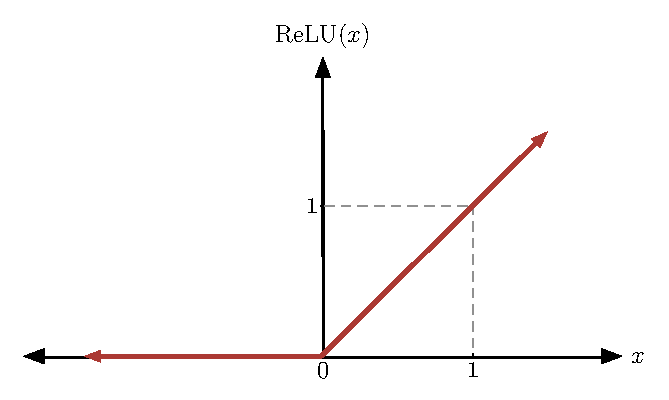
\includegraphics[width=.7\textwidth]{images/relu.pdf}
    \caption{$\RELU$ non linearity visualized.}
    \label{fig:relu}
  \end{centering}
\end{figure}


As \cite{glorot2011deep} explained, $\RELU$ leads to sparsity. As a result, given an input, only a subset of nodes are non-zero (active) and every possible subset results with a linear function. This linearity allows a better flow of gradients, leading to faster training. Also, the $\RELU$ is easier to compute compared to hyperbolic or exponential alternatives.

We will redefine the fully connected $\FC$ with activation function ($\sigma$) as
$$ \FCk{k}(\ok{k}) = \sigma((\ok{k})^T\wk{k} + \bk{k})$$

The activation function does not strictly belong to the definition of fully connected layers. But for simplicity, we are going to include them in the layer functions ($\psi$).

$\FC$ is one of the most basic building blocks of neural networks. By stacking building blocks in different types and configurations, we come up with different neural network structures. The outputs of every layer, starting from the input are calculated as
$$ \all\outputvar = \{\lfk{k}(\ok{k-1}) \ | \  k \in [1, \ldots, \num\layer] \} $$
% And we will describe the whole operation with a function $\nnfunc$, such that, 
% $$\nnfunc : \x \rightarrow \yh$$
\subsection{Loss}

To represent the quality of an approximation, we are going to use a loss (or cost) function. A good example to understanding loss would be the loss of a salesman. Assuming a customer who would pay at most \$10 for a given product, if the salesman sells this product for \$4, the salesman would face a loss of \$6 from his potential profit. Or if the salesman tries to sell this product for \$14, the customer will not purchase it and he will face a loss of \$10. In this example, the salesman would want to minimize the loss to earn as much as possible. There are two common properties of loss functions. First, loss is never negative. Second, if we compare two approximations, the one with smaller loss is better at approximating the data.

\subsubsection{Root Mean Square Error}
A commonly used loss function is root mean square error ($\RMSE$). Given an approximation ($\yhn{n} \inreal{N}$) and the expected output ($\yn{n} \inreal{N}$), $\RMSE$ can be calculated as
\begin{equation*}
\loss = \RMSE(\yhn{n}, \yn{n}) = \sqrt{\frac{\sum^N_{i=1} (\yhni{n}{i} - \yni{n}{i})^2 }{N}}
\end{equation*}

\subsubsection{Softmax Cross Entropy}
Another commonly used loss function is softmax cross entropy ($\SCE$). Softmax cross entropy is used for classification tasks where we are trying to find the class that our input belongs to. Softmax cross entropy first calculates the class probabilities given the input using the softmax function. It is defined as

$$p(i | \yhn{n}) = \frac{e^{\yhni{n}{i}}}{\sum_{j=1}^{N}e^{\yhni{n}{j}}}$$
Then comparing it with the the expected output ($\yn{n} \inreal{N}$), $\SCE$ loss can be calculated as
$$\loss = \CE(\yhn{n}, \yn{n}) = - \sum_{i=1}^{N} \yni{n}{i} log(p(i | \yhn{n}))$$

$\SCE$ depends on the softmax to turn the node outputs into probabilities. Therefore, it makes sense to use it for classification tasks where the output data is representing a probability distribution. However, $\RMSE$ punishes the difference in outputs. Therefore, we can say that it is better for tasks like regression which represent exact values in output nodes. \cite{golik2013cross} provides a comprehensive comparison of both methods. 

\subsection{Minimizing Loss}
To provide better approximations, we will try to optimize the neural network parameters. One common way to optimize these parameters is to use stochastic gradient descent (SGD). SGD is an iterative learning method that starts with some initial (random) parameters. Given $\theta \in (\all\weights \cup \all\biasterm$) to be a parameter that we want to optimize. The learning rule assigning the new value of $\theta$ for a simple example would be

$$ \theta := \theta- \eta \nabla_\theta{\loss(f(\x),\y)} $$
where $\eta$ is the learning rate, and $\nabla_\theta{\mathcal{L}(f(x), y)}$ is the partial derivative of the loss in terms of the given parameter ($\theta$) and $:=$ is the assignment operator. One iteration is completed when we update every parameter for given example(s). By performing many iterations, SGD aims to find a global minimum for the loss function, given data and initial parameters.

There are several other optimizers that work in different ways. We will be using Momentum Optimizer (\cite{qian1999momentum}) and SGD.

\subsection{Convolutional Layer}
So far we have seen the key elements we can use to create and train fully connected neural networks. To be able to apply neural networks to image inputs, we can define convolutional layers using convolution operations. 

Let us assume a 3 dimensional layer output $\ok{k-1} \inreal{\heightk{k-1} \times \widthk{k-1} \times \mk{k-1}}$ where the dimensions $\heightk{k-1}$ representing the length of the height dimension, $\widthk{k-1}$ representing the length of the width dimension and $\mk{k-1}$ representing number of nodes in that layer. We will refer to the totality of these nodes repeated in width and height dimensions as features or channels. Convolution operation first creates a sliding window of size $\kernelsize \times \kernelsize \times \mk{k-1}$ that goes through height and width dimensions. The contents of this sliding window are patches ($\pki{k-1}{(I,J)} \inreal{\kernelsize \times \kernelsize \times \mk{k-1}}$) where $0 < I \leq \widthk{k}$ and $0 < J \leq \widthk{k}$. By multiplying the weight matrix $\wk{k} \inreal{\kernelsize \times \kernelsize \times \mk{k-1} \times \mk{k}}$ to the patch $\pki{k-1}{(I,J)}$  centered at $(I,J)$, we create the set of output nodes for that point $\oki{k}{(I,J)} \inreal{1 \times \mk{k}}$. While calculating the patches, we also make use of a parameter called stride, $\sk{k} \in \mathbb{N}^+$. $\sk{k}$ defines the number of vertical and horizontal steps to take between each patch.

In other words, strides ($\sk{k}$) are used to define the width ($\widthk{k}$) and height ($\heightk{k}$) of the output in layer $k$ as
$$ \widthk{k} = \floor*{\frac{\widthk{k-1}}{\sk{k}}}, \heightk{k} = \floor*{\frac{\heightk{k-1}}{\sk{k}}}$$
Using this relationship between dimensions of outputs, we can define a convolutional layer as
$$ \convk{k} : \imagedimsk{k-1} \rightarrow \imagedimsk{k} $$
To perform this operation, we need to define and create the patch at location $(I,J)$ as 
$$ \pki{k-1}{(I,J)} \inreal{\kernelsize \times \kernelsize \times \mk{k-1}} $$
$$ \pki{k-1}{(I,J)} \subseteq \ok{k-1}$$

The subindices ($i,j$) of patch ($\pki{k-1}{(I,J)}$) are a direct reference to the features at subindex ($a,b$) of the output. Using these indices, elements of this patch are defined as
$$ \pki{k-1}{(I,J),(i,j)} \inreal{\mk{k-1}} , 0 < i \leq \kernelsize, 0 < j \leq \kernelsize$$
$$ \oki{k-1}{a,b} \inreal{\mk{k-1}} , 0 < a \leq \heightk{k-1}, 0 < b \leq  \widthk{k-1} $$
This direct reference is
$$ \pki{k-1}{(I,J),(i,j)} = \oki{k-1}{a,b} $$
where the relationship between subindices of the output layer ($a,b$) and the patch ($(I,J),(i,j)$) are defined dependent on the strides and the kernel size as
$$ a = I\sk{k} + (i - \floor*{\kernelsize/2}) $$
$$ b = J\sk{k} + (j - \floor*{\kernelsize/2}) $$

In cases where $a$ and $b$ become less than 0 (i.e. $i=0, I=0$) or greater than $\heightk{k-1}$ and $\widthk{k-1}$ respectively, we assign zeroes to relative values of the patches. This method is called \textit{same padding}, and we will be using this method for the rest of our definitions. 

Having the definition for a patch $\pki{k-1}{(I,J)}$ and the indices related to it, we can define the output of the next layer as
$$\convk{k}(\ok{k-1}) = \ok{k} = \{\oki{k}{(I,J)} \ | \ \forall (I,J) (\exists \pki{k-1}{(I,J)}) [ \oki{k}{(I,J)} = \sigma(\pki{k-1}{(I,J)} \wk{k} + \bk{k})\ \}  $$
where the weight and the bias are defined as
$$ \wk{k} \inreal{\kernelsize \times \kernelsize \times \mk{k-1} \times \mk{k}} $$
$$ \bk{k} \inreal{\mk{k}}$$
\begin{figure}[!h]
  \begin{centering}
    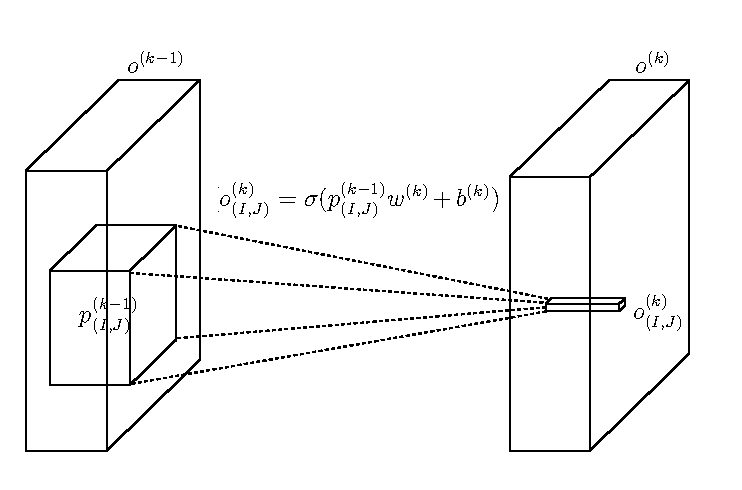
\includegraphics[width=1\textwidth]{images/convolution.pdf}
    \caption{Convolution operation visualized. }
    \label{fig:convolution}
  \end{centering}
\end{figure}
In other words, as shown in Figure~\ref{fig:convolution}, the output of layer is a set of vectors ($\ok{k} = \{\oki{k}{(I,J)}\}$). For every pair of indices ($I,J$), there exists a patch $\pki{k-1}{(I,J)}$ defined by the outputs of the previous layer. We apply the weight, the bias and the activation function to these patches to calculate the set $\ok{k}$. Given this description, we can define the complexity of this operation as
$$ \bigo{\convk{k}} = \bigo{\widthk{k}\heightk{k}\kernelsize^2\mk{k-1}\mk{k}} $$



\subsection{Pooling}
Just like strides, pooling is another way of reducing the dimensionality ($\width{k}$ and $\height{k}$) of a layer. Depending on the task, one may choose from different pooling methods. Similar to convolution operation, pooling methods also work with patches $\pki{k-1}{(I,J)} \inreal{\kernelsize \times \kernelsize \times \mk{k-1}}$ and strides $\sk{k-1}$. But this time, instead of applying a weight, bias and activation function, they apply simpler functions. Here we will see two types of pooling layers.

\subsubsection{Max Pooling}
Max pooling takes the maximum value in a channel within the patch. Let's define the first subindex of a patch as if it is referring to a node as
$$ \pki{k-1}{(I,J),i} \inreal{\kernelsize \times \kernelsize}, 0 < i \leq \mk{k-1} $$
Using this definition, max pooling can be defined as
$$ \maxpoolk{k}(\ok{k-1}) = \ok{k} = \{ \oki{k}{(I,J),i} \ | \ \forall ((I,J),i) (\exists \pki{k-1}{(I,J),i}) [\oki{k}{(I,J),i} = \max(\pki{k-1}{(I,J),i})]  \}  $$

In other words, for every index $(I,J),i$, there exists a $K \times K$ matrix. The value of the output at index $(I,J),i$ is defined as the maximum value of that matrix. Max pooling is mostly used after the first or second convolutional layer to reduce the dimensionality of the input in classification tasks.

\subsubsection{Average Pooling}
Average pooling averages the values within the patch per channel. The subindices of patch $\pki{k-1}{(I,J)}$ are defined as
$$ \pki{k-1}{(I,J),i,a,b} \inreal{} $$
Using this definition, average pooling can be defined as
$$ \avgpoolk{k}(\ok{k-1}) = \ok{k} = \{\oki{k}{(I,J),i}  \ | \ \forall ((I,J),i) (\exists\pki{k-1}{(I,J),i}) [\oki{k}{(I,J),i} = \sum_{a=1}^{\kernelsize}\sum_{b=1}^{\kernelsize}\frac{\pki{k-1}{(I,J),i,a,b}}{\kernelsize^2} ]\} $$
In other words, for every index $(I,J),i$, there exists a $K \times K$ matrix. The value of the output at index $(I,J),i$ is defined as the average value of that matrix. 

\subsubsection{Global Pooling Methods}
Global pooling methods take the output layer as one patch and reduce height and width dimensions to a single channel by applying the target function (max or average). Global average pooling is mostly used before the last fully connected layers in classification tasks.

\subsection{Deconvolution}
Introduced by \cite{zeiler2010deconvolutional}, deconvolution operation aims to increase the dimensionality of an input. To do that, it basically transposes the convolution operation. Deconvolution operation creates patches of $\pki{k-1}{(I,J)} \inreal{1 \times 1 \times \mk{k-1}}$ from the input, and applies a weight matrix of $\wk{k} \inreal{\mk{k-1} \times \kernelsize \times \kernelsize \times \mk{k}}$. In other words, it creates a $\kernelsize \times \kernelsize \times \mk{k}$ output from every $1 \times 1 \times \mk{k-1}$ patch and expands the height and width of the input. 

\subsection{Batch Normalization}
\cite{ioffe2015batch} introduced a method called batch normalization. Batch normalization aims to normalize the output distribution of every node in a layer. By doing so it allows the network to be more stable. 

Assume the layer k with $\ok{k} \inreal{\mk{k}}$ where $\mk{k}$ is the number of nodes. Batch normalization has four parameters. Mean is $\mu^{(k)} \inreal{\mk{k}}$, variance is $\sigma^{(k)} \inreal{\mk{k}}$, scale is $\gamma^{(k)} \inreal{\mk{k}}$ and offset is $\beta^{(k)} \inreal{\mk{k}}$. 

Since we are interested in normalizing the nodes, even if $k$ was a convolutional layer, the shapes of these parameters would not change. Therefore, batch normalization function $\textrm{BN}$ can be defined as 
$$ BN(\ok{k}) = \frac{\gamma^{(k)}(\ok{k}-\mu^{(k)})}{\sigma^{(k)}}+\beta^{(k)} $$

\subsection{Regularization}
Regularization methods aim to prevent overfitting in neural networks. Overfitting is the case where the weights of a a neural network converge for the training dataset. Meaning that the network performs very good for the training dataset, while it is not generalized to work with any other data. Regularization methods try to prevent this.

One common regularization method is to add a new term to the loss, which influence the weight in certain ways. We also add a term $\lambda$ which determines the effect of this regularization. Setting $\lambda$ too high will influence the gradient descent steps more than the data itself. In such a case, we may end up with a non-optimal solution. Setting $\lambda$ too low will reduce the effects of regularization. We look at two types of regularizers, L1 and L2. 

\subsubsection{L1 Regularization}
L1 regularization pushes regularized values towards zero. Therefore, it is good to force the weights to become small or very close to zero. L1 regularization is defined as
$$ L1 = \lambda \sum_{w \in \mathbf{W}} |w| $$ 

\subsubsection{L2 Regularization}
L2 regularization punishes values with a square term. Therefore, L2 regularization pushes the weights towards zero. However, it pushes the values that are greater than one or minus one more than the values in between. L2 regularization is defined as
$$ L2 = \lambda \sum_{w \in \mathbf{W}} w^2 $$


\iffalse
\section{Efficient Structures}
Some structures help neural networks represent more information using fewer parameters. We are going to look at some structures that are known to work well with convolutional neural networks.

\subsection{Residual Blocks}
\cite{He:2015aa} introduced two types of residually connected blocks. The first is called a residual block, consisting of two convolution operations and a residual connection between the input and the output of the block. The second is called a residual bottleneck block, consisting of three convolution operations. First reducing number of channels with a one by one kernel, second applying a three by three kernel, third applying another one by one kernel to increase the number of dimensions. \cite{He:2015aa} have used residual blocks to train networks up to 34 layers. For networks having 50 or more layers, they have used the residual bottleneck block. Their 50-layer network using residual bottleneck blocks achieves $22.85\%$ top-1 error rate on ImageNet dataset while their 34-layer network is achieving $25.3\%$ top-1 error rate.
\fi
\iffalse
\subsection{Residual Bottleneck Blocks}
Residual bottleneck blocks consist of three convolution operations with different kernel sizes and number of output nodes. 

Before explaining how residual bottleneck blocks are configured, we need more notations to define the layers inside the same block. Let us assume the block $b$ with input $o_{b-1} \inreal{H_{b-1} \times W_{b-1} \times \mk{b-1}}$. We will index the layers inside the block $b$ with a pair $(b, k)$ where $k$ stands for the index of convolutional layer inside the block. For example, if we're talking about the second convolutional layer in block $b$, the input of this convolutional layer would be $o_{(b, 1)} \inreal{H_{(b, 1)} \times W_{(b, 1)} \times \mk{(b, 1)}}$ and the output would be $o_{(b, 2)} \inreal{H_{(b, 2)} \times W_{(b, 2)} \times \mk{(b, 2)}}$. also since we are talking about layers with different kernel sizes, we need to define them with indexes as well. Therefore the kernel size of convolutional layer $(b,k)$ would be $K_{(b,k)} \in \mathbb{R}$.
Therefore, we can define the residual bottleneck block as;
$$ \psi_b^{(ResidualBottleneck)}: \real{H_{b-1} \times W_{b-1} \times \mk{b-1}} \rightarrow  \real{H_{b} \times W_{b} \times \mk{b}} $$
with the helper function $S$
$$ \psi_b^{(ResidualBottleneck)}(o) =  S(o) + \psi_{(b, 3)}^{(Conv)}(\psi_{(b, 2)}^{(Conv)}(\psi_{(b, 1)}^{(Conv)}(o))) $$
\begin{equation*}
    S_b(o) = 
\begin{cases}
    o, &\text{if } (W_b, H_b, m_b) = (W_{b-1}, H_{b-1}, \mk{b-1})\\
    P_b(M_b^{(avg)}(o)),& \text{otherwise}\\
\end{cases}
\end{equation*}
where $P$ is a padding function that equalizes the number of nodes in the outputs and $M_b^{(avg)}$ is the average pooling function that equalizes the width and height dimensions of the input and output of the block.
To their definition the first convolution operation in the block reduces the number of nodes with kernel size $K_{(b,1)}=1$. The number of nodes is defined with a dependency to the stride of block ($s_b \in \{1,2\})$ as $\mk{(b,1)} = \mk{b}/(4/s_b)$. By that logic, if a residual block is reducing the width and height by half, it is doubling the number of nodes to represent more information. Second convolution operation kernel size $K_{(b,2)}=3$ and has the same number of nodes as the previous layer $\mk{(b,2)} = \mk{(b,1)}$. The third convolutional layer quadruples the number of nodes ($\mk{(b,3)} = 4\mk{(b,1)}$) with kernel size $K_{(b,3)} = 1$.

\fi

\iffalse
\begin{table}[]
\centering
\begin{tabular}{ | c | c | c | c | }
\hline
layer name			& output size 					& 34-layer																& 50-layer																			\\ \hline
input image			& $224 \times 224$				& \multicolumn{2}{c|}{}																																	\\ \hline
conv1				& $112 \times112$				& \multicolumn{2}{c|}{$ 7 \times 7$, $64$, stride $2$}																												\\ \hline
\multirow{2}{*}{conv2\_x}	& \multirow{2}{*}{$56 \times 56$} 	& \multicolumn{2}{c|}{$3 \times 3$ max pool, stride $2$}																											\\ \cline{3-4} 
					&							& $\begin{bmatrix} 3 \times 3, &   64 \\ 3 \times 3, &   64 \end{bmatrix} \times 3 $		& $\begin{bmatrix}1 \times 1, & 64 \\ 3 \times 3, & 64 \\ 1 \times 1, & 256 \end{bmatrix}^{} \times 3 $ 		\\ \hline
conv3\_x				& $28 \times 28$				& $\begin{bmatrix} 3 \times 3, & 128 \\ 3 \times 3, & 128 \end{bmatrix} \times 3 $		& $\begin{bmatrix}1 \times 1, & 128 \\ 3 \times 3, & 128 \\ 1 \times 1, & 512 \end{bmatrix} \times 3$		\\ \hline
conv4\_x				& $14 \times 14$				& $\begin{bmatrix} 3 \times 3, & 256 \\ 3 \times 3, & 256 \end{bmatrix} \times 3 $		& $\begin{bmatrix}1 \times 1, & 256 \\ 3 \times 3, & 256 \\ 1 \times 1, & 1024 \end{bmatrix} \times 3$		\\ \hline
conv5\_x				& $  7 \times   7$				& $\begin{bmatrix} 3 \times 3, & 512 \\ 3 \times 3, & 512 \end{bmatrix} \times 3 $		& $\begin{bmatrix}1 \times 1, & 512 \\ 3 \times 3, & 512 \\ 1 \times 1, & 2048 \end{bmatrix} \times 3$		\\ \hline
					& $  1 \times   1$				&\multicolumn{2}{c|}{average pool, 1000-d fc, softmax}																											\\ \hline
\multicolumn{2}{| c |}{FLOPs}							& $3.6 \times 10^9$														& $3.8 \times 10^9$																	\\ \hline
\multicolumn{2}{| c |}{top-1 error ($\%$)}						& $21.53$																& $20.74$																			\\ \hline
\multicolumn{2}{| c |}{top-5 error ($\%$)}						& $5.60$																& $5.25$																			\\ \hline
\multicolumn{2}{| c |}{top-1 error \small{($\%$, \textbf{10-crop} testing)}}						& $24.19$																& $22.85$																			\\ \hline
\multicolumn{2}{| c |}{top-5 error \small{($\%$, \textbf{10-crop} testing)}}						& $7.40$																& $6.71$																			\\ \hline
\end{tabular}
\caption{Comparison of bottleneck blocks (50-layer) with stacked $ 3 \times 3$ layers (34-layer). }
\label{tab:bottleneck-comparison}
\end{table}
\fi

\section{Datasets}
In this section we will see the datasets that we have experimented with. Since we are mostly focusing on convolutional neural networks, we will look at 3 image classification datasets.

\subsection{MNIST}
MNIST dataset \cite{lecun1998mnist} consists of 60.000 training and 10.000 test samples. Each sample is a $28 \times 28$ black and white image of a handwritten digit ($0$ to $9$). To our knowledge, the best model trained on MNIST achieve almost zero ($0.23\%$, \cite{DBLP:journals/corr/abs-1202-2745}) error rate. 

\subsection{CIFAR10}
CIFAR10 dataset \cite{krizhevsky2009learning} consists of 50.000 training and 10.000 test samples. Each sample is a $32 \times 32$ colored image belonging to one of 10 classes. The classes are airplane, automobile, bird, cat, deer, dog, frog, horse, ship and truck. To our knowledge, the best model trained on CIFAR10 achieve $3.47\%$ (\cite{DBLP:journals/corr/Graham14a}) error rate.

\subsection{ImageNet}
The dataset used in ILSVRC is called ImageNet. ImageNet \cite{deng2012image} comes with $1.281.167$ training images and $50.000$ validation images consisting of $1000$ classes containing multiple dog species and daily objects. ImageNet comes with bounding boxes showing where the object is in the image. We are interested in the object detection task. So we crop these bounding boxes and feed them to our neural network for training. The best submission from 2016 challenge has achieved $0.02991$ error rate. This is equal to $97.009\%$ top-5 accuracy. 
\iffalse
\section{Inference on Mobile Devices}
We will be comparing the inference speed of various models using mobile devices. Mobile devices a great benchmarking platform because they have great availability all around the world. There are two major factors determining the inference speed of a model.

\subsection{Floating Point Multiplications}
Floating point multiplications are more complicated than addition operations. Therefore addition operations can be considered irrelevant compared to the multiplications. A model that has a low total number of floating point multiplications is expected to have a faster inference speed.

\subsection{Model Size}
Modern processors have a memory hierarchy. The first element in this hierarchy is the register. The processor can access the values that are in the register effortlessly. After register there is the processor cache layer. Cache layer has a larger size than the register. But accessing values in the cache layer is more expensive than the register layer. In the hierarchy after the cache layer, there is the memory layer. The memory layer is much larger than the cache layer, but it is much more expensive for the processor to access this data. 

Therefore as the model size grows, the lack of moving information from memory to cache would increase. In some cases, this operation would cause the processor to wait before performing an instruction. Such a case is called as the "memory bandwidth bottleneck". To minimize the effects of memory bandwidth bottleneck, we need to stick with smaller networks. In theory if we can come up with a model that fits the cache layer, we could increase the inference speed greatly. In practice, that depends on the implementation of the neural network.

\section{Tools}
\subsection{Tensorflow}
To develop and train our neural networks, we used Tensorflow \cite{abadi2016tensorflow}. Tensorflow provides us the necessary tools to deploy our trained models on mobile devices. 
\fi
